\documentclass{poly}
\usepackage{main}

\title{Dérivation locale et globale}
\author{Terminale STMG1}
\date{}

\begin{document}
\maketitle
\section{Définition de la fonction dérivée}
\begin{remark}
Soit $f$ une fonction définie sur un intervalle $I$, dont la courbe représentative est notée $\mathcal{C}_f$. Soit $a \in I$, on note $A(a;f(a))$ un point de la courbe $\mathcal{C}_f$. La tangente à la courbe $\mathcal{C}_f$ en $A$ (quand elle existe), est une droite passant par $A$ et \og frôlant \fg la courbe $\mathcal{C}_f$. 
\end{remark}
\begin{center}
\begin{tikzpicture}
\tikzmath{\xmax = 6.25; \ymax = 4.25;}
\draw[help lines] (-\xmax, -\ymax) grid[step=0.5] (\xmax,\ymax);
\draw[->,thick] (-\xmax,0) -- (\xmax,0) node[right] {$x$};
\draw[->,thick] (0,-\ymax) -- (0,\ymax) node[above] {$y$};
\clip (-\xmax,-\ymax) rectangle (\xmax,\ymax);
\draw[thick] plot[samples=100] (\x,{0.5*\x^3 + 2*\x*\x - 3});
\draw (-2,1) node {$\bullet$} node[above right] {$A$};
\draw[thick] (-4,5) -- (4,-11);
% y = -2(x + 2) + 1
\end{tikzpicture}
\end{center}
\begin{exercize*}
Placer deux points $B$ et $C$ sur la courbe $\mathcal{C}_f$, puis tracer les deux tangentes à $\mathcal{C}_f$ en $B$ et $C$.
\end{exercize*}
\begin{definition}
Soit $f$ une fonction définie sur un intervalle $I$. On dit que la fonction est \textbf{dérivable} sur $I$ si pour tout $a \in I$, la courbe représentative de $f$, $\mathcal{C}_f$ admet une tangente en $A(a;f(a))$.
\end{definition}
\begin{definition}
Soit $f$ une fonction définie et dérivable sur $I$. Alors, on appelle $f'$ la \textbf{fonction dérivée de $f$} la fonction définie sur $I$ qui à tout $a \in I$ associe la pente de la tangente de $\mathcal{C}_f$ en $A(a;f(a))$.
\end{definition}
\newpage
\begin{remark}
Étant donné une fonction $f$, déterminer si $f$ est dérivable et calculer sa fonction dérivée $f'$ le cas échéant permet d'évaluer les variations de $f$. En effet, le tableau de signe de $f'$ permet d'établir le tableau de variation de $f$.
\end{remark}
\begin{exercize*}
Soit $f : x \mapsto x^3 - 9x^2 + 24x$ définie sur $\R$. On admet que $f$ est dérivable sur $\R$ et que sa fonction dérivée est donnée par
\begin{equation*}
f' : x \mapsto 3x^2 - 18x + 24
\end{equation*}
\begin{alphaquestions}
\item Montrer que pour tout $x \in \R$,
\begin{equation*}
f'(x) = 3(x-2)(x-4)
\end{equation*}
\item Compléter le tableau de signe de $f'$ puis en déduire le tableau de variation de $f$.
\begin{center}
\begin{tikzpicture}
\tkzTabInit{$x$/1, Signe de $(x-2)$/1, Signe de $(x-4)$/1, Signe de $f'$/1, Variation de $f$/2}{$-\infty$, $2$, $4$, $+\infty$};
\tkzTabLine{,,z,,};
\tkzTabLine{,,,,z,};
\tkzTabLine{,,z,,z,};
\end{tikzpicture}
\end{center}
\end{alphaquestions}
\end{exercize*}
\section{Calcul de dérivée}
\begin{proposition}
Soit $f$ une fonction définie sur $\R$ telle que, pour $x \in \R$, $f(x)$ est de la forme
\begin{equation*}
f(x)=a_nx^n + a_{n-1}x^{n-1} + \dots + a_1x + a_0
\end{equation*}.
Alors, $f$ est dérivable sur $\R$, et sa dérivée vaut, pour tout $x \in \R$,
\begin{equation*}
f'(x) = a_nnx^{n-1} + a_{n-1}(n-1)x^{n-2} + \dots + a_1
\end{equation*}
\end{proposition}
\begin{example}
Vérifier que la fonction $f : x \mapsto x^3 + 5x^2 - 4x + 2$ est dérivable, puis calculer sa dérivée.
\end{example}
\end{document}